\subsection{Antarmuka Halaman Registrasi}    
    Halaman ini dapat diakses oleh semua pengguna, baik yang belum terdaftar maupun sudah. Halaman ini menampilkan form berisi elemen \textit{input} data diri, dan pengguna dapat mengisi lalu mengklik tombol daftar, dan untuk kasus alternatif dapat dilihat pada Tabel \ref{uc01.01}.\\
	\indent Tidak ada \textit{view logic} ataupun logika \textit{UI} khusus dalam halaman ini. Kode sumber implementasi \textit{back-end} dapat dilihat pada Kode Sumber \ref{cdbe.01-01}.

  \begin{figure}[H]
    \centering
    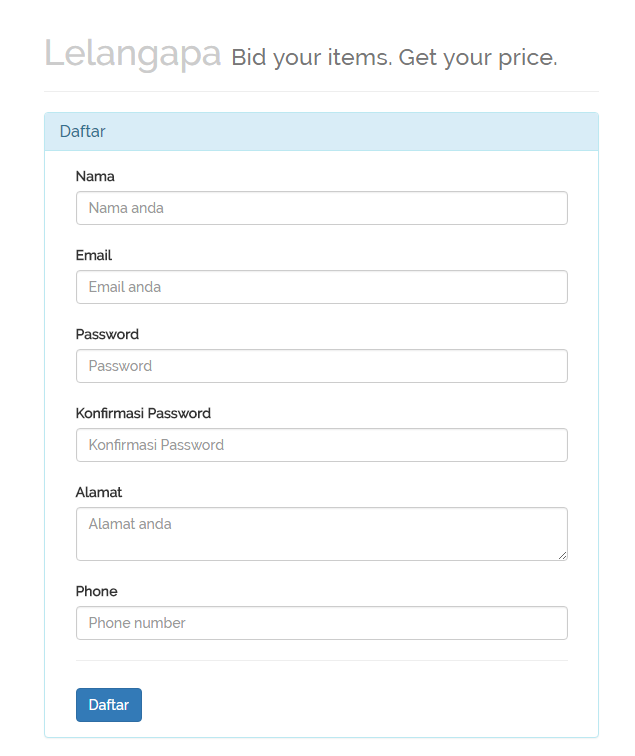
\includegraphics[width=\textwidth]{images/bab4/ui/01-01.png}
    \caption{Halaman antarmuka registrasi}
    \label{ui.01-01}
  \end{figure}
  
\begin{lstlisting}[label=cdbe.01-01,style=php,caption=Kode Sumber Antarmuka Registrasi]
/* 
 * Menampilkan halaman register
 * method : GET 
 */
public function showRegistrationForm(){
	
	return view('auth.register2');
}

/*
 * validator fungsi 
 */
protected function validator(array $data){
	
	return Validator::make($data, [
		'name' => 'required|max:255',
		'email' => 'required|email|max:255|unique:users',
		'password' => 'required|min:6|confirmed',
		'username' => 'required|unique:users|min:5',
		'phone' => 'numeric',
	]);
}

 /*	
  * Dipanggil saat mengklik tombol daftar
  * method : POST 
  */
public function register(Request $request){

				
	/*	validasi data */
	$this->validator($request->all())->validate();

	event(new Registered($user = $this->create($request->all())));

	$this->guard()->login($user);

	/* notify activationService 
	to send activation mail to user's email */
	$this->activationService->sendActivationMail($user);

	return $this->registered($request, $user) ?
	   : redirect($this->redirectPath());
	 
}
	  
	  
\end{lstlisting}
	  
      
      